% Información para el motor (arara). Compilar en LuaLaTeX o XeLaTeX sólamente.

% arara: lualatex: {
% arara: --> interaction: nonstopmode,
% arara: --> options: ['-file-line-error'],
% arara: --> shell: yes,
% arara: --> synctex: yes,
% arara: --> }
% arara: makeglossaries
%% arara: makeindex

\documentclass[letterpaper,12pt,twoside,es-MX]{article}

% %%%%%%% VARIABLES ESTÁTICAS %%%%%%%
% Aqui se definen las variables para diferentes procedimientos.
% Verificar que las unidades coincidan si se deciden cambiar.

\newcommand{\defglo}[1]{\item[{\bfseries \glsname{#1}}] \glsdesc{#1}} % Define un comando para dar un item en un entorno de descripción para una palabra definida en el glosario
% \includeonly{src/PSA-2.19.tex,src/PSA-Gloss.tex}
\newcommand{\TipoID}{TEMP} % Definirlo como: PRO, PROG, ToC, G, L, CE, CI, I, etc.
\newcommand{\Prog}{TEMP}
\newcommand{\ProgTitulo}{TEMP}

\newcommand{\ie}{\emph{i.e.}}
\newcommand{\eg}{\emph{e.g.}}

%%%%%%%%%%%%%%%% Formularios %%%%%%%%%%%%%%%%
\newcommand{\IdFormAACC}{F-OP-40}

\newcommand{\BitES}{Bitácora de entradas y salidas --- Clientes (F-AD-1)}
\newcommand{\BitULl}{Bitácora de uso de llaves (F-AC-1)}
\newcommand{\BitVig}{Bitácora de vigilancia (F-AC-2)}
\newcommand{\Fpap}{Papeleta (F-AC-3)}
\newcommand{\Oent}{Orden de entrada (F-AC-4)}
\newcommand{\Osal}{Orden de salida (F-AC-5)}
\newcommand{\LayES}{Layout de carga o descarga (F-AC-6)}
\newcommand{\BitClor}{Bitácora de cloración de agua (F-AC-7)}
\newcommand{\BitTap}{Bitácora de concentración de tapete sanitario (F-AC-8)}
\newcommand{\BitUQ}{Bitácora de uso de productos químicos (F-AC-9)}
\newcommand{\BitLAd}{Bitácora de limpieza de aduana sanitaria (F-AC-10)}
\newcommand{\BitLOf}{Bitácora de limpieza de oficinas (F-AC-11)}
\newcommand{\BitLEx}{Bitácora de limpieza de exteriores (F-AC-12)}
\newcommand{\BitBPH}{Bitácora de cumplimiento de BPH (F-HyS-1)}
\newcommand{\BitCAP}{Bitácora de consumo de agua potable (F-HyS-2)}
\newcommand{\BitCE}{Bitácora de consumo de energía eléctrica (F-HyS-3)}
\newcommand{\BitIEx}{Bitácora de inspección de extintores (F-HyS-4)}
\newcommand{\BitVIR}{Bitácora de verificación de termómetros infrarrojos (F-HyS-5)}
\newcommand{\LVCMo}{Lista de verificación de condición de montacargas (F-HyS-6)}
\newcommand{\RTAC}{Registro de temperaturas con termómetro IR --- Aseguramiento de calidad (F-HyS-7)}
\newcommand{\RTMa}{Registro de temperaturas con termómetro IR --- Mantenimiento (F-HyS-8)}
\newcommand{\RAcL}{Registro de actividad de limpieza (F-HyS-9)}
\newcommand{\RAcM}{Registro de actividad de mantenimiento (F-Hys-10)}
\newcommand{\ReEq}{Registro de revisión de equipos de enfriamiento (F-MAN-1)}
\newcommand{\RCMi}{Registro de inspección de infraestructura en prevención (F-MAN-2)}
\newcommand{\Rcap}{Registro de asistencia a capacitación (F-MAN-3)}
\newcommand{\REvDQ}{Registro de eventos de derrame de químicos (F-MAN-4)}
\newcommand{\InvVyPD}{Registro de inventario de vidrio y plástico duro (F-MAN-5)}
\newcommand{\RVerSGC}{Registro de verificación del sistema de gestión de calidad (F-MAN-6)}
\newcommand{\RRCA}{Registro de recorrido de control de alérgenos (F-MC-1)}
\newcommand{\RAC}{Registro de acción correctiva o preventiva (F-OP-1)}
\newcommand{\RACQ}{Registro de acción correctiva --- Quejas (F-OP-2)}
\newcommand{\RVSCP}{Registro de verificación del servicio de control de plagas (F-OP-3)}
\newcommand{\RevD}{Registro de revisión diaria (F-SEG-1)}
\newcommand{\RCVyPD}{Registro de evento de contaminación por VyPD (F-SEG-2)}
\newcommand{\REvCA}{Registro de evento de contaminación por alérgeno (F-SEG-3)}



%%%%%%%%%%%%%%%% CÓDIGOS PSA %%%%%%%%%%%%%%%%
% \newcommand{\PSA}{PSA-3-PRO}                 % PSA-2.3 Inspección de producto durante su almacenamiento

%%%%%%%%%%%%%%%% PSA-2.3 | Inspección de producto durante su almacenamiento %%%%%%%%%%%%%%%%
\newcommand{\TiempoAndenCong}{\qty{\leq 30}{\minute}}
\newcommand{\TiempoAndenRefri}{\qty{\leq 30}{\minute}}
\newcommand{\TiempoAveriaRefri}{4}              % Tiempo máximo de permanencia de alimento refrigerado en cámara averiada (en horas) 
\newcommand{\TiempoAveriaConge}{10}             % Tiempo máximo de permanencia de alimento congelado en cámara averiada (en horas)
\newcommand{\EspacioMinimoParedProducto}{30}    % Espacio entre tarima y pared (en centimetros)
\newcommand{\EspacioMinimoTechoProducto}{30}    % Espacio entre tarima y techo (en centimetros)
\newcommand{\VecesTempManual}{dos}              % Veces que se verifica la temperatura manualmente



%%%%%%%%%%%%%%%% PSA-2.3 | Política de aprobación de proveedores %%%%%%%%%%%%%%%%
\newcommand{\NotifAuditoriaAProveedor}{2 semanas}           % Plazo máximo para notificar a proveedor sobre auditoría.
\newcommand{\PlazoResultadoAProveedor}{2 semanas}           % Plazo máximo para notificar a proveedor sobre resultados de auditoría.
\newcommand{\PlazoPlanDeAccionAuditProveedor}{2 semanas}    % Plazo maximo para recibir plan de acción de parte del proveedor tras auditoría

%%%%%%%%%%%%%%%% PSA-2.15 | Almacenamiento de registros %%%%%%%%%%%%%%%%
\newcommand{\VigenciaAlmacRegistros}{2 años}
\newcommand{\VigenciaAlmacRegistrosElec}{3 años}

%%%%%%%%%%%%%%%% GLOBAL | Resetear glosarios en cada sección %%%%%%%%%%%%%%%%
\usepackage{etoolbox}
\preto\section{\glsresetall}

\newcommand{\AC}{aseguramiento de calidad}
\newcommand{\G}{gerencia}
\newcommand{\AD}{alta dirección}
\newcommand{\OP}{operaciones}
\newcommand{\Emb}{embarques}
\newcommand{\MC}{mesa de control}     % Definición de variables estáticas
                                        % i.e. Tiempo máximo de cámras de refrigeración sin energía



%%%%%%%%%%%%%%%%%%%%%%%%%%% ESPECIALES %%%%%%%%%%%%%%%%%%%%%%%%%%%%%%%%%%
\RequirePackage{expl3}    % \usepackage cannot be used before \documentclass
\ExplSyntaxOn             % Switch on expl3 syntax
\pdf_version_gset:n{1.7}  % Use provided expl3 function
\ExplSyntaxOff            % Switch off expl3 syntax

%%%%%%%%%%%%%%%%%%%%%%%%%%% Tipografía %%%%%%%%%%%%%%%%%%%%%%%%%%%%%%%%%%

\usepackage[sfdefault,t,lf]{carlito}    % Alternativa OpenSource a Calibri, definir sans serif como predeterminado, numerales tabulares
% \usepackage[default,lnum]{opensans}
% \usepackage{CormorantGaramond}
% \usepackage{fontspec}
% \setmainfont{Carlito}

\usepackage{polyglossia}
	\setdefaultlanguage[variant=mexican,spanishoperators=all]{spanish}  % Definir la localización del documento como es-MX (para que cuadro sea tabla, etc.)

\usepackage{changelog}  % Control de versiones

\usepackage[toc=true,postpunc={;},showtargets=annoteleft,style=tree,xindy]{glossaries-extra}    % Manager de glosarios, usar xindy para el indice alfabético
	\makeglossaries                             % Hacer que arara haga glosarios
	\setabbreviationstyle[acronym]{long-short}  % Estilo de acrónimos
	\loadglsentries[main]{./glosario-def.tex}  % Archvio que LuaLaTeX toma para las definiciones

\usepackage{imakeidx}       % Para hacer indices
	\makeindex[columns=2]   % Estilo del indice alfabético

\newcounter{note}[section]  % Nuevo contador para notas
\renewcommand{\thenote}{\thesection.\Alph{note}}    % Definir estilo de numeración de las notas
\usepackage[framemethod=TikZ]{mdframed}             % Motor gráfico para notas (TikZ)
\newenvironment{note}[1][]{%                        % Nuevo entorno de Nota (note) 
    \refstepcounter{note}
    \begin{mdframed}[%                                  
        frametitle={Nota \thenote\ #1},                 % Titulo de las notas
        skipabove=\baselineskip plus 2pt minus 1pt,     % Espaciado superior
        skipbelow=\baselineskip plus 2pt minus 1pt,     % Espaciado inferior
        linewidth=0.5pt,                                % Tamaño de linea del recuadro
        frametitlerule=true,                            % incluir titulo
        frametitlebackgroundcolor=gray!30               % Color del recuadro
    ]%
}{%
    \end{mdframed}
}

\newcounter{contact}[section]                           % Nuevo contador para contactos
\renewcommand{\thecontact}{\thesection.\Alph{contact}}  % Definir que la numeración sea Sección.Alfabético

\newenvironment{contact}[1][]{%
    \refstepcounter{contact}
    \begin{mdframed}[%
        frametitle={Contacto \thecontact\ #1},          % Titulo del contacto
        skipabove=\baselineskip plus 2pt minus 1pt,     % Espaciado superior
        skipbelow=\baselineskip plus 2pt minus 1pt,     % Espaciado inferior
        linewidth=0.5pt,                                % Tamaño de linea del recuadro
        frametitlerule=true,                            % poner titulo
        frametitlebackgroundcolor=yellow!30             % Color del recuadro
    ]%
}{%
    \end{mdframed}
}

\usepackage[multiple]{footmisc}     % Cambios en la presentación de pies de página
\usepackage{microtype}              % Ajustes de kerning y otros 
\usepackage{graphicx}               % Mejora al motor de imagenes
\usepackage{hyperref}               % Referencias cruzadas en PDF
\usepackage{cleveref}               % Referencias cruzadas en texto
%%%%%% REDEFINICIONES DE REFERENCIAS CRUZADAS %%%%%%%%%
    \crefname{note}{nota}{notas}    
	\Crefname{note}{Nota}{Notas}
	\crefname{contact}{contacto}{contactos}
	\Crefname{contact}{Contacto}{Contactos}
	\crefname{paragraph}{parrafo}{parrafos}
	\Crefname{paragraph}{Parrafo}{Parrafos}
%%%%%%%%%%%%%%%%%%%%%%%%%%%%%%%%%%%%%%%%%%%%%%%%%%%%%%%
\newcommand{\email}[1]{\href{mailto:#1}{#1}}    % Comando para hacer que se puedan clickear emails
\newcommand{\cels}[1]{\qty{#1}{\celsius}}       % Escrir celsius rapido

\usepackage{lastpage}   % Definir variable para el numero total de páginas
\usepackage{siunitx}    % Unidades internacionales y alineamiento de decimales en tablas
	\sisetup{detect-all}    % Detectar automaticamente que la tipografía es sans serif

\usepackage{color}  % definir colores nuevos

\usepackage{tabularray} % Creación de tablas
	\UseTblrLibrary{booktabs,siunitx}   % librerias parea tablas correctas, unidades internacionales
	\definecolor{Gallery}{rgb}{0.929,0.929,0.929}   % definición del color "Gallery"
	\DefTblrTemplate{contfoot-text}{normal}{\textit{Continúa en la siguiente página}}   % Continuación de tabla
	\SetTblrTemplate{contfoot-text}{normal} % Continuación de tabla normal (footer)
	\DefTblrTemplate{conthead-text}{normal}{\textit{(Continuación)}}    % Continuación de tabla
	\SetTblrTemplate{conthead-text}{normal} % Continuación de tabla (header)

    % \usepackage[margin=1cm,bmargin=2cm,tmargin=5cm,headheight=110pt]{geometry}   % Dispoción espacial del documento
% \newgeometry{includeheadfoot, heightrounded, left=1cm, right=1cm, top=1cm, bottom=4cm, headheight=6em, footskip=1.5em}    
%     \savegeometry{L1}

% \newgeometry{includeheadfoot, heightrounded, left=1cm, right=1cm, top=1cm, bottom=4.5cm, headheight=7em, footskip=1.5em, showcrop, showframe}
%     \savegeometry{L2}

\usepackage[%
includeheadfoot,
heightrounded,
left=1cm,
right=1cm,
top=1cm,
bottom=1cm,
headheight=110pt,
footskip=1.5em]{geometry}    



\usepackage{enumitem}
	\setlist[1]{labelindent=\parindent} % Indentación como parrafo para listas
	\setlist[itemize]{leftmargin=*} % Eliminar margen en izq
	\setlist[itemize,1]{label=---}  % Viñeta como em-dash
	\setlist{noitemsep} % Que no se separen los item

%%%%%%%%%%%%%%%% DEFINICIÓN DE CABECERA %%%%%%%%%%%%%%%%
\usepackage{fancyhdr}   % Usar fancy headers y footers
	\renewcommand{\headrulewidth}{0pt}  % Grosor de regla del header
	\fancyhead[CE,CO,LE,LO,RE,RO]{} % Resetear headers    
    \fancyfoot[CE,CO,LE,LO,RE,RO]{} % Resetear footers

    %%%%%%%%%%%%%%%%%%%%%% VARIABLES DE CADA DOCUMENTO DENTRO DE UN PROGRAMA %%%%%%%%%%%%%%%%%%%%%
	\newcommand{\Codigo}{}                  % Codigo del documento
	\newcommand{\FechaPub}{}                % Fecha de publicación
	\newcommand{\Titulo}{}                  % Titulo del documento
	\newcommand{\MayorVer}{}                % Versión mayor
	\newcommand{\MenorVer}{}                % Verisón menor
	\newcommand{\Edit}{\MayorVer.\MenorVer} % Definición de la edición

    \newcommand{\Elaboro}{}                 % Nombre de quien lo elaboró
    \newcommand{\Reviso}{}                  % Nombre de quien revisó el documento
    \newcommand{\Autorizo}{}                % Nombre de quien aprobó el documento
    %%%%%%%%%% Formato por defecto para informaicón documentada general %%%%%%%%%%

\fancypagestyle{PrimeraPag}{%
    \fancyhead[C]{%
	    \raisebox{4em}[0pt][0pt]{%
            \begin{tblr}{%	
            colspec = {X[c,m]X[c,m]X[c,m]X[c,m]X[c,m]X[c,m]},    % Especificación de columnas: Anchura estática, centrado en medio
            hlines,
            vlines,
            }
            \SetCell[c=2]{c} 
\includegraphics[height=1cm]{./RDF_Logo.png} & & \SetCell[c=3]{c} \large{Red de fríos S.A. de C.V.} & & & {\textbf{Código:}\\ \Codigo} \\ % Logotipo (2 columnas), red de frios (3 columnas), código del documento
            \SetCell[c=4]{c} {Titulo:\\ \Titulo} & & & & {\textbf{Fecha de publicación:}\\ \FechaPub} & {\textbf{Edición:}\\ \Edit} \\ % Titulo (4 columnas), Fecha, edición
            \end{tblr}
	    }%
    }%
}%
    % \fancyfoot[L,C,R]{}
    % \fancyfoot[C]{%
    % \raisebox{-4em}[0pt][0pt]{%
    %     \begin{tblr}{%	
    %         colspec = {X[c,m]X[c,m]X[c,m]},    % Especificación de columnas: Anchura estática, centrado en medio
    %         hlines,
    %         vlines,
    %         }%
    %             Elaboró & Revisó & Autorizó  \\
    %             \vspace{1cm} & & \\
    %             \Elaboro & \Reviso & \Autorizo 
    %     \end{tblr}
    % }%
    % }%
% }%
% \setlength{\footskip}{40pt}

\fancypagestyle{formato-PS}{%
\fancyhead{}
\fancyfoot{}
    \fancyhead[RE]{%
	    \begin{tblr}{%	
            colspec = {X[c,m]X[c,m]},    % Especificación de columnas: Anchura estática, centrado en medio
            hlines,
            vlines,
            width = 0.35\linewidth,
            }%
            {\textbf{Código:}\\ \Codigo} & {\textbf{Edición:}\\ \MayorVer.\MenorVer} \\ % Logotipo (2 columnas), red de frios (3 columnas), código del documento
            {\textbf{Fecha de publicación:}\\ \FechaPub} & {Página \thepage\ de \pageref{LastPage}} % Titulo (4 columnas), Fecha, edición
            \end{tblr}
    }%

    \fancyhead[LO]{%
        \begin{tblr}{%	
            colspec = {X[c,m]X[c,m]},    % Especificación de columnas: Anchura estática, centrado en medio
            hlines,
            vlines,
            width = 0.35\linewidth,
            }%
            {\textbf{Código:}\\ \Codigo} & {\textbf{Edición:}\\ \MayorVer.\MenorVer} \\ % Logotipo (2 columnas), red de frios (3 columnas), código del documento
            {\textbf{Fecha de publicación:}\\ \FechaPub} & {Página \thepage\ de \pageref{LastPage}} % Titulo (4 columnas), Fecha, edición
        \end{tblr}
    }%

    \fancyfoot[C]{Página \thepage\ de \pageref{LastPage}}   % Para que muestre Página # de #
    \fancyfoot[L]{\textbf{CONFIDENCIAL}}                    % CONFIDENCIAL
    \fancyfoot[R]{\Codigo~v.\Edit}                          % Estructura del código CODIGO v.EDICION
}%
    

\fancypagestyle{formato-PI}{%
\fancyhead{}
\fancyfoot{}
    \fancyhead[C]{%
	    \begin{tblr}{%	
            colspec = {X[c,m]X[c,m]X[c,m]X[c,m]X[c,m]X[c,m]},    % Especificación de columnas: Anchura estática, centrado en medio
            hlines,
            vlines,
            }%
            \SetCell[c=2]{c} 
\includegraphics[height=1cm]{./RDF_Logo.png} & & \SetCell[c=3]{c} \large{Red de fríos S.A. de C.V.} & & & {\textbf{Código:}\\ \Codigo} \\ % Logotipo (2 columnas), red de frios (3 columnas), código del documento
            \SetCell[c=4]{c} {Titulo:\\ \Titulo} & & & & {\textbf{Fecha de publicación:}\\ \FechaPub} & {\textbf{Edición:}\\ \Edit} \\ % Titulo (4 columnas), Fecha, edición
            \end{tblr}
	    }%
    %%%%%%%%%%%%%% Definición de Footers %%%%%%%%%%%%%%%%
    \fancyfoot[C]{Página \thepage\ de \pageref{LastPage}}   % Para que muestre Página # de #
    \fancyfoot[L]{\textbf{CONFIDENCIAL}}                    % CONFIDENCIAL
    \fancyfoot[R]{\Codigo~v.\Edit}                          % Estructura del código CODIGO v.EDICION
}%

%%%%%%%%%%%%%%%%%%%%%%%%%%%%%%%%%%%%%%%%%%%%%%%%%%%%%%%%%

\setcounter{tocdepth}{4}            % Qué tanto mostrará la tabla de contenidos
\setcounter{secnumdepth}{6}         % Que tantas secciones numerará LaTeX (Se ajustó hasta subparrafo)

 % Define un comando para dar un item en un entorno de descripción para una palabra definida en el glosario


\begin{document}
\pagestyle{formato-PS}
\thispagestyle{formato-PI}
\renewcommand{\MayorVer}{1}
\renewcommand{\MenorVer}{0}
\renewcommand{\Codigo}{\textbf{TEMP}-ToC}
\renewcommand{\FechaPub}{2023-03}
%\renewcommand{\Edit}{01}
\renewcommand{\Titulo}{\textbf{TEMP} --- Índice}

\tableofcontents
\listoftables   % Tabla de contenidos, figuras y tablas
% \thispagestyle{PrimeraPag}
% includeheadfoot, heightrounded, left=1cm, right=1cm, top=1cm, bottom=1cm, headheight=7em, footskip=1.5em]
% \newgeometry{includeheadfoot, heightrounded, left=1cm, right=1cm, top=1cm, bottom=1cm, headheight=7em, footskip=1.5em, showcrop, showframe}
% \savegeometry{Alt}
\thispagestyle{formato-PI}

\renewcommand{\Elaboro}{XXXX}
\renewcommand{\Reviso}{YYYY}
\renewcommand{\Autorizo}{ZZZZ}
\renewcommand{\MayorVer}{3}             % Renovar comando, Versión mayor
\renewcommand{\MenorVer}{0}             % Renovar comando, Versión menor
\renewcommand{\Codigo}{PRO-AC-101}      % Renovar comando, código del documento
\renewcommand{\FechaPub}{2023--01}      % Renovar comando, Fecha de publicación
\renewcommand{\Titulo}{Elaboración y control de documentos} % Renovar comando, Titulo del documento

\section{\Titulo}   % Sección = Titulo definido en la linea anterior
\index{Información documentada!tipo!procedimiento!Elaboración y control de documentos}  % Como se encontrará en el indice
\index{Procedimientos!Elaboración y control de documentos}                              % Como se encontrará en el indice

\subsection{Objetivo}
Asegurar que los \glspl{documento} del \gls{SGC} se preparan, revisan, aprueban, publican, distribuyen, implementan y administran de acuerdo a lo especificado en este procedimiento.

\subsection{Alcance}
Este procedimiento aplica a todos los documentos generados internamente por cada uno de los departamentos o de fuentes externas y personal involucrado en la elaboración, consulta y actualización de documentos en el \gls{SGC}

\subsection{Terminología y definiciones}
\index{Procedimientos!Elaboración y control de documentos!Terminología y definiciones}
\begin{description}
    \item[\glsname{copia-controlada}] \glsdesc{copia-controlada} 
    \item[\glsname{copia-no-controlada}] \glsdesc{copia-no-controlada} 
    % De ahora en delante se usará el comando definido por el usario como \defglo{} para eficientizar el tiempo
    % NOTA: Debe de estar incluido en el archivo del glosario la definición a introducir (Ver linea 242 del template)
    \defglo{documento-interno}
    \defglo{listado-maestro}
    \defglo{procedimiento-estandar}
    \defglo{procedimiento-estandar-de-limpiesza}
    \defglo{instruccion-de-trabajo}
    \defglo{especificacion}
    \defglo{anexo}
    \defglo{formato}
    \defglo{registro}
\end{description}

\subsection{Responsabilidades}
\index{Procedimientos!Elaboración y control de documentos!Responsabilidades}
\subsubsection{Aseguramiento de calidad}
\begin{itemize}
    \item Coordina y verifica que se lleve a cabo la actualización en tiempo y forma de los documentos y registros del Sistema de Calidad.
    \item Administra la totalidad de documentos del Sistema de Calidad.
    \item Asigna la numeración correspondiente a los documentos elaborados.
    \item Responsable de la aprobación, revisión y emisión de documentos de acuerdo con su área de responsabilidad.
\end{itemize}

\subsubsection{Gerente de mantenimiento}
\begin{itemize}
    \item Responsable de la elaboración, actualización, revisión, emisión y aplicación de los documentos generados en su área, así como de los documentos del Sistema de Calidad donde tenga injerencia.
\end{itemize}

\subsubsection{Gerente de operaciones}
\begin{itemize}
    \item Responsable de la elaboración, actualización, revisión, emisión y aplicación de los documentos generados en su área, así como de los documentos del Sistema de Calidad donde tenga injerencia.
\end{itemize}

\subsubsection{Jefe de higiene y sanidad}
\begin{itemize}
    \item Responsable de la elaboración, actualización y aplicación de los documentos generados en su área, así como de los documentos del Sistema de Calidad donde tenga injerencia.
\end{itemize}

\subsection{Procedimiento}
\subsubsection{Generación de Documentos} \label{GenDeDoc}
Determinar la necesidad de documentar y validar con el jefe inmediato del área. Identificar el tipo de documento necesario a generar y proceder a documentar y/o generar el documento en base a los siguientes lineamientos:
\paragraph{Estructura}
\subparagraph{Encabezado}
Todos los documentos deben contenerlo y debe incluir:
\begin{itemize}
    \item Logotipo
    \item Título del documento
    \item Código de identificación del documento
    \item Revisión actual del documento
    \item Fecha de emisión
\end{itemize}

\subparagraph{Código}
El código de identificación del documento está formado de la siguiente manera:
La primera parte consta de 1 a 3 letras, las cuales indican el tipo de documento de acuerdo con la \cref{tbl:1.1}

\begin{longtblr}[%
    label = {tbl:1.1},
    caption = {Categorías según el tipo de información documentada},
    ]{%
    width = 0.35\linewidth,
    colspec = {Q[c,m]Q[c,m]},
    row{even} = {Gallery},
    }
    \toprule
        Código & Tipo de documento \\ \midrule
        LM     & Listado Maestro   \\
        PRO    & Procedimiento     \\
        F      & Formatos          \\
        PR     & Programa          \\
        PO     & Política          \\
        RE     & Reglamento        \\
    \bottomrule
\end{longtblr}

La segunda parte consta de dos letras correspondientes al área que genera el documento (no es limitativo), ver \cref{tbl:1.2}

\begin{longtblr}[%
label = {tbl:1.2},
caption = {Categorías según el área operativa},
]{%
width = 0.35\linewidth,
colspec = {Q[c,m]Q[c,m]},
row{even} = {Gallery},
}
\toprule
GE	& Gerencia \\ \midrule
AC	& Aseguramiento de Calidad \\
MA	& Gerencia de Mantenimiento \\
OP	& Gerencia de Operaciones \\
TR	& Departamento Transportes \\
HS	& Departamento Higiene y Sanidad \\
\bottomrule
\end{longtblr}

Los últimos dos dígitos (dos) indican el número consecutivo del documento del área  departamento. Se inicia con el número uno.

\emph{Ejemplo:} 

\begin{center}
PRO-AC-01
\end{center}

\begin{longtblr}[%
label = {tbl:1.3},
caption = {Ejemplo de la codificación de un documento},
]{%
width = 0.35\linewidth,
colspec = {Q[c,m]Q[c,m]},
row{even} = {Gallery},
}
    \toprule
        PRO	& Procedimiento \\ \midrule
        AC 	& Aseguramiento de Calidad \\
        01	& Número de Documento \\ 
    \bottomrule
\end{longtblr}

\subparagraph{Edición}
Indica el número de veces que el documento ha sido modificado y/o adecuado, se inicia con el número que corresponde a la primera emisión.

\subparagraph{Fecha de Publicación}
Corresponde a la fecha en que el documento se elaboró

\subparagraph{Contenido}
Corresponde a la información que contiene el documento y como debe ser presentada.
\begin{enumerate}
    \item \textbf{Objetivo:} Finalidad para la cual fue creado el documento.
    \item \textbf{Alcance:} Áreas o puestos para los cuales es aplicable el documento.
    \item \textbf{Terminología y Definiciones:} Conjunto de términos o palabras propias utilizadas en un procedimiento.
    \item \textbf{Responsabilidades:} Indica los compromisos de los participantes en el desarrollo de un documento.
    \item \textbf{Procedimiento:} Desarrollo de la actividad o proceso a seguir paso a paso.
    \item \textbf{Frecuencia:} Es la frecuencia con la que se debe realizar cada actividad.
    \item \textbf{Documentos Relacionados:} Todos los documentos con relación al procedimiento.
    \item \textbf{Anexos:} Agregados de un trabajo que se incluyen al final del documento y ofrecen información adicional. 
    \item \textbf{Formatos:} Todos los formatos con relación al procedimiento.
    \item \textbf{Historial de modificaciones:} Muestra cuál ha sido el histórico de las modificaciones o adecuaciones que ha tenido el documento. Se establece la revisión anterior, revisión actual, fecha de las revisiones y una descripción de las modificaciones realizadas.
    \item \textbf{Listado de Distribución:} Lista donde se menciona a quien se le ha compartido el procedimiento o documento y cuenta con copia.
\end{enumerate}

\subparagraph{Tipo de letra}
Los documentos se deben desarrollar con base a la estructura del presente documento y deben ser escritos en letra Calibri 12 pt. Los títulos deben ser en negrilla, combinando mayúsculas y minúsculas.

\subparagraph{Numeración}
Inicie el esquema de numeración partiendo del número 1 y según se requiera, desglose el mismo agregando un punto y un decimal, \emph{por ejemplo:} 1, 1.1, 1.1.1. De ser necesario en cada punto utilicé incisos y /o viñetas.

\subparagraph{Revisar el documento elaborado, para asegurar que se cumplen todos los puntos para la estandarización; que incluye el formato, estructura y contenido.}
\subparagraph{Llevar a cabo la ruta de aprobación del documento}
\subparagraph{Si el documento es aprobado proceder a la difusión e implementación del mismo.}
\subparagraph{Los formatos tienen como mínimo (cuando aplique)}
\begin{itemize}
    \item Código 
    \item Revisión
    \item Titulo 
    \item Numero de hojas
    \item Firma de la(s) persona(s) responsable(s) de llenar el registro
    \item Firma de autorización y/o verificación
\end{itemize}

\subparagraph{Los registros son llenados en cada uno de sus espacios, cuando un espacio no es utilizado, por no ser necesario se coloca una línea horizontal o diagonal para cancelarlo.}

\subparagraph{Todos los documentos y registros deben resguardarse de manera que no sufran daño y/o deterioro.}

\subsubsection{Revisión y aprobación de Documentos} \label{RevApDoc}
\begin{enumerate}
\item Si el documento presenta faltas de cumplimiento al presente procedimiento, la persona responsable de la revisión notifica al puesto que generó el documento para que proceda a realizar las modificaciones señaladas y repita las actividades a partir del punto 
\item Si el documento fue aprobado por los involucrados en la ruta de aprobación se procede a su difusión e implementación.
\end{enumerate}

\subsubsection{Distribución, implementación y control de Documentos}
\begin{enumerate}
    \item Los documentos aprobados serán incluidos con la codificación correspondiente en el Listado Maestro de documentos para su control.
    \item Ya liberado el documento (emisión inicial o cambios) el Jefe de Aseguramiento de Calidad realizará las copias y distribuirá el documento de acuerdo a 12 Listado de Distribución.
    \item Cuando se requiera una copia física de los documentos aprobados y vigentes, se realiza una solicitud a Aseguramiento de Calidad, cada copia deberá ser sellada como se indica en la \cref{an1} según corresponda.
    \item Para solicitar  documentos con copia no controlada, se tiene que mandar una solicitud por escrito al Jefe de Aseguramiento de Calidad especificando el motivo de la solicitud.
\end{enumerate}

\subsubsection{Cambios, alta o baja de documento}
\begin{enumerate}
    \item Para realizar cambios, alta o baja de documentos se debe seguir y cumplir los pasos de la \cref{GenDeDoc} al \cref{RevApDoc} Se debe informar a Aseguramiento de Calidad a través del formato O-F-RCP Solicitud de Alta, Baja o Cambio de documentos. \cref{an2}
    \begin{enumerate}
        \item Cambiar el contenido del documento según los cambios necesarios para adecuarlo al  proceso y/o revisar la propuesta de cambio que haga el área solicitante.
        \item Cambiar la revisión de los documentos (Procedimientos, Instructivos o registros).
        \item Llenar el punto 10 del procedimiento, Historial de Cambios, con las especificaciones generales del cambio.
        \item Actualizar el Listado Maestro.
        \item Para finalizar, el Jefe de Aseguramiento de Calidad imprime el documento autorizado y comienza el proceso de distribución y difusión (ver punto 5.3).
    \end{enumerate}
    \item Cuando se realice algún cambio, se debe actualizar el punto 7.0 Historial de Modificaciones del Documento, este punto muestra cual ha sido el histórico de las modificaciones o adecuaciones que ha tenido el documento.
\end{enumerate}

\subsubsection{Control de documentos obsoletos}
\begin{enumerate}
\item Todo documento tiene  1 año de vigencia. Posterior a esta fecha se debe realizar una revisión, para asegurar que la información es actual y corresponde al proceso y/o actividad que se ejecutan.
\item Retire de los puntos de uso los documentos obsoletos que haya distribuido físicamente de acuerdo al listado de distribución y remplace el documento por la revisión vigente para que el personal involucrado siempre tenga la versión actualizada para ejecutar sus actividades; asegure que todos los documentos obsoletos sean retirados y remplazados.
\item Destruya las copias de los documentos obsoletos y destrúyalos conservando un ejemplar que se identificará con la leyenda de DOCUMENTO OBSOLETO (Véase \cref{an-d}) y consérvelos en base a los lineamientos de Control de Registros. (5.1.14).
\end{enumerate}

\subsubsection{Respaldo de la información}
\begin{enumerate}
    \item La documentos electrónicos del Sistema de Calidad es respaldada por el Jefe de Aseguramiento de Calidad con una frecuencia mensual
\end{enumerate}

\subsection{Frecuencia}
\begin{enumerate}
\item Cada vez que sea necesaria la publicación o modificación de algún documento del sistema de calidad.
\end{enumerate}

\subsection{Documentos relacionados}
\begin{itemize}
    \item Todos los documentos y/o procedimientos relacionados al sistema de calidad.
\end{itemize}

\subsection{Formatos}
\begin{itemize}
    \item Formato de cambio de procedimiento \emph{O-F-RCP}
\end{itemize}

\begin{changelog}[simple, sectioncmd=\subsection*,label=changelog-1.1]
	\begin{version}[v=3, date=2023--03--06]
		\item N/A.
	\end{version}

	\begin{version}[v=2, date=2022--03--02]
		\item Cambio de anexos para incluir sellos de control.
	\end{version}

    \begin{version}[v=1, date=2021--09--14]
		\item Origen del documento.
	\end{version}
\end{changelog}

\appendix
\newpage
\section{Sellos para el control documental}

\begin{figure}[h!]
    \centering
    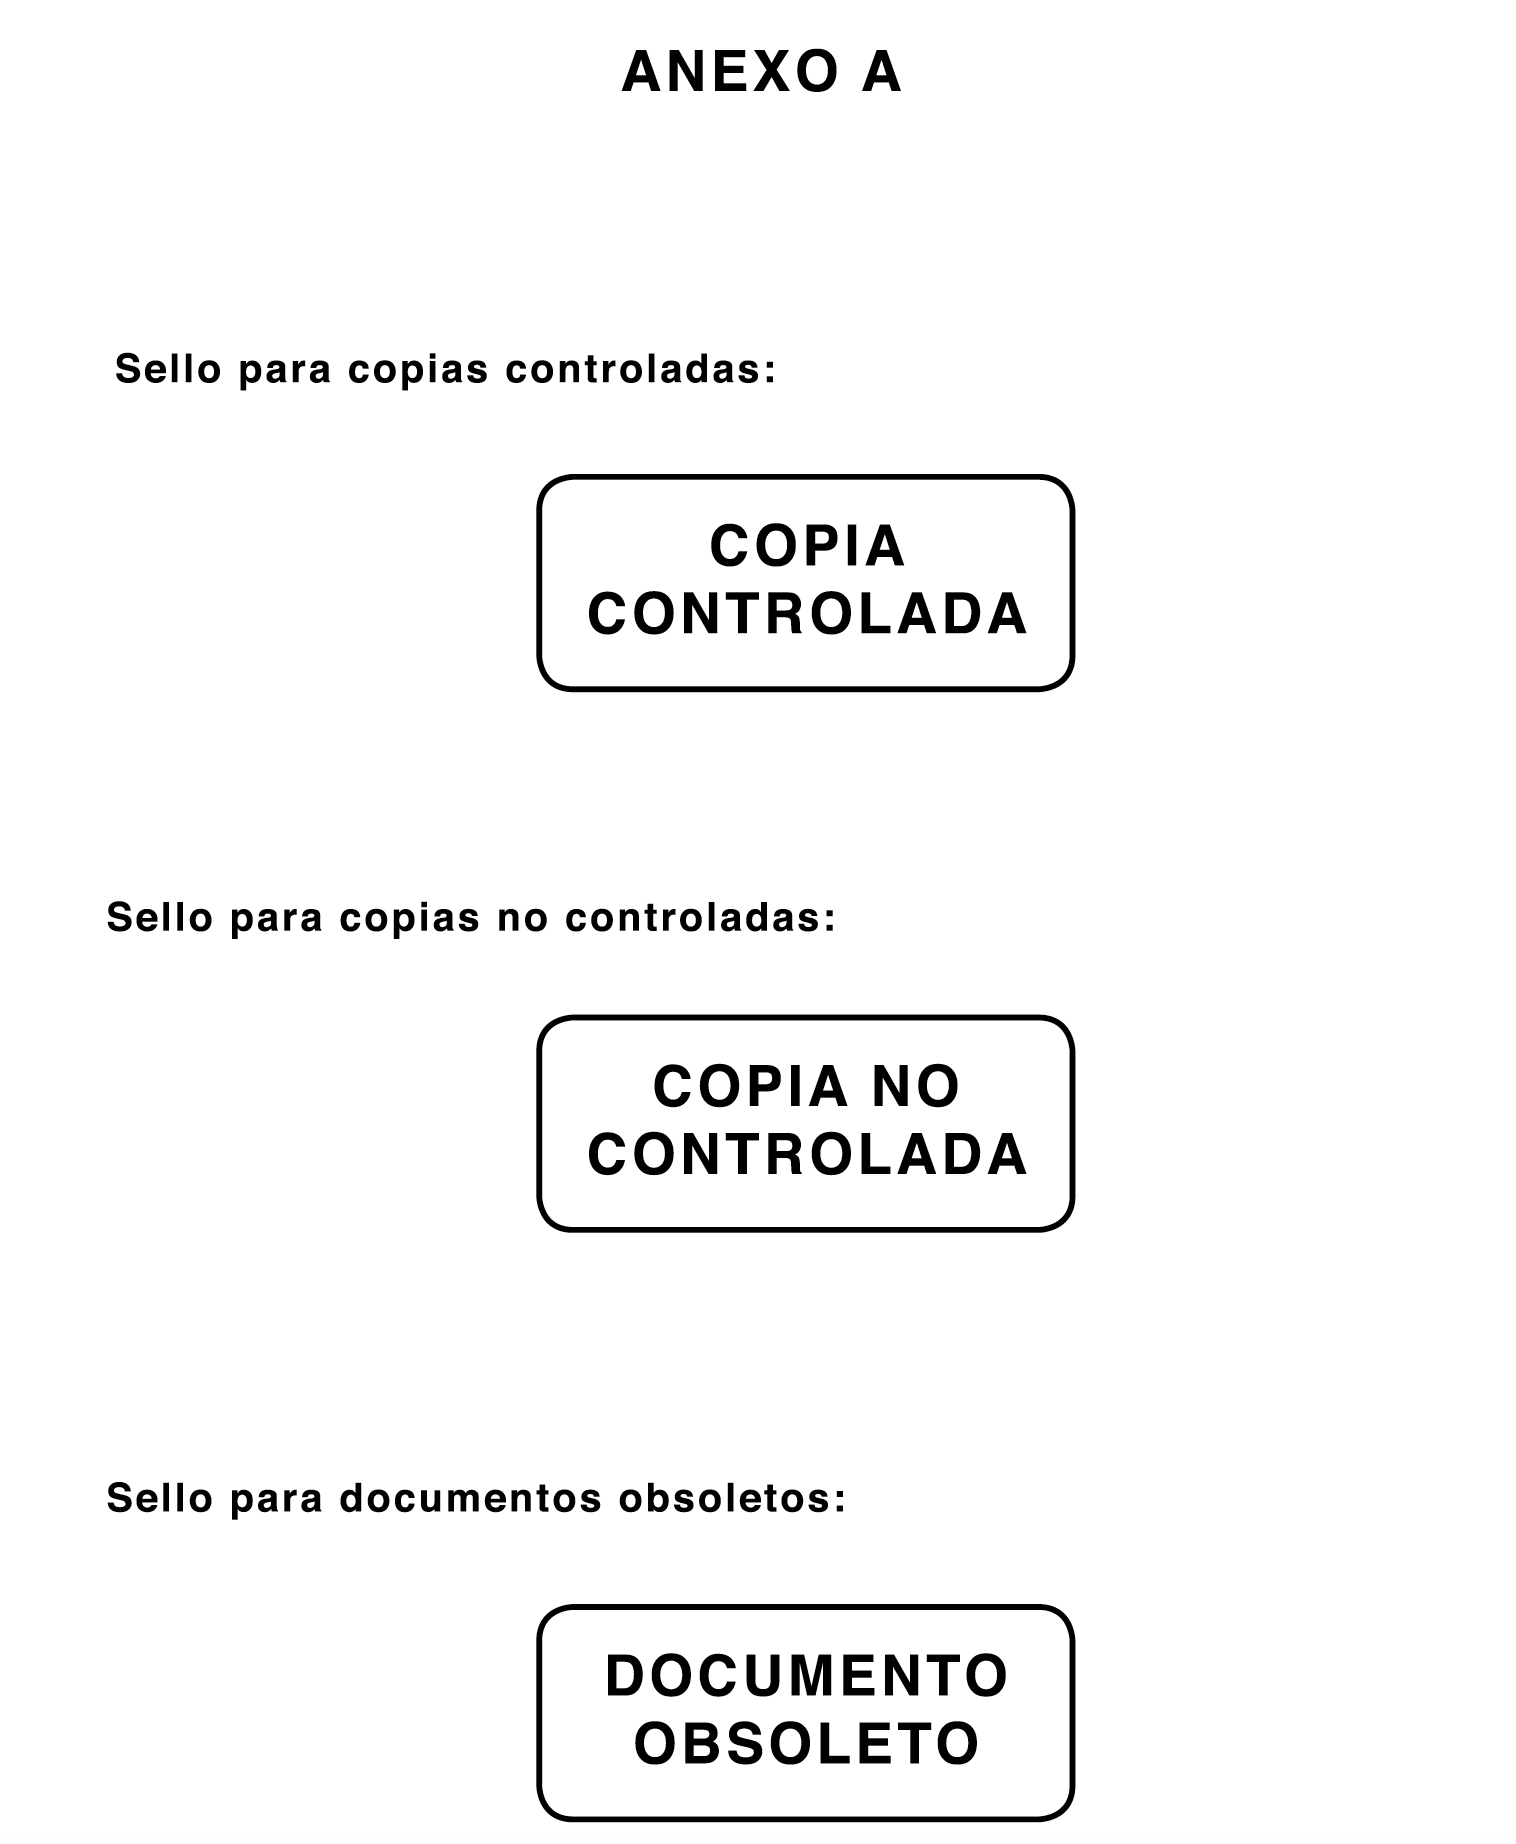
\includegraphics[width=0.5\linewidth]{A1.png}
    \label{an1}
    \caption{Sellos empleados para controlar documentos}
\end{figure}

  % Documento 1 de carpeta X
\thispagestyle{formato-PI}
\renewcommand{\MayorVer}{1}
\renewcommand{\MenorVer}{0}
\renewcommand{\Codigo}{\textbf{TEMP}-ToC}
\renewcommand{\FechaPub}{2023--01}
%\renewcommand{\Edit}{01}
\renewcommand{\Titulo}{\textbf{TEMP} --- Glosario}

\printglossary % Glosario de las palabras empleadas en todo este documento
\end{document}